\chapter{Interaction discovery for logistic regression} \label{chap5}

\epigraph{.}{.}

\minitoc


\textcolor{red}{needs quote}

\textit{Nota Bene :} Ce chapitre s'inspire fortement ... \textcolor{red}{à adapter au moment de l'envoi du manuscrit}

\bigskip

\selectlanguage{english}

Continuing my pursuit of interpretable representation learning algorithms for logistic regression, I tackle in this chapter a common problem in \textit{Credit Scoring} and other application contexts relying either on logistic regression or additive models of the form $g(y) = \sum_{j=1}^d \glssymbol{bth}_j' \q_j(x_j)$. To further reduce the model bias discussed in Section~\ref{chap1:sec3} and thus obtain better predictive performance while maintaining interpretability, \textit{Credit Scoring} practitioners are used to introducing pairwise interactions.


\section{Motivation: XOR function}

As described in the introduction, logistic regression is linear in its inputs which does not allow to take into account conditional dependency, see~\cite{berry2010testing}. This problem is often dealt with by sparsely introducing ``interactions'', \textit{i.e.}\ products of two features. Unfortunately, this leads again to a model selection challenge as the number of pairs of features is $\dfrac{d(d-1)}{2}$. We denote by $\bdelta$ the upper triangular matrix with $\delta_{k,\ell} = 1$ if $k < \ell$ and features $k$ and $\ell$ ``interact'' in the logistic regression in the sense of~\cite{berry2010testing}. The logistic regression with interactions $\bdelta$ is thus:
\begin{equation} \label{eq:reglog_sans}
\text{logit}[p_{\glssymbol{bth}}(1|\q(\glssymbol{bx}),\bdelta)] = \theta_{0} + \sum_{j=1}^d \glssymbol{bth}_j' \q_j(x_j) + \sum_{1 \leq k < \ell \leq d} \delta_{k,\ell} \glssymbol{bth}_{k,\ell} \odot \q_k(x_k) \q_\ell(x_\ell)',
\end{equation}
where $\odot$ denotes the element-wise matrix multiplication, $\glssymbol{bth}_{k,\ell} = (\theta_{k,\ell}^{r,s})_{1 \leq r \leq m_k, 1 \leq s \leq m_\ell}$ and for all features $j$, $m_j$ is set as the ``reference'' value and consequently for all $j$, $\theta_{j}^{m_j}=0$ and for all $1 \leq k < \ell \leq d$, $\theta_{k,\ell}^{m_k,m_{\ell}}=0$.

This formulation seems rather complicated visually and in terms of parameter dimension: a single interaction between two quantized features (or more broadly speaking, categorical features) amounts to adding $m_k \cdot m_\ell$ coefficients. Since we advocated ``interpretable'', \textit{i.e.}\ sparse, simple models to yield scorecards as in Table~\ref{tab:ex_scorecard}, and we witnessed a high variance when estimating numerous coefficients on Figure~\ref{fig:sinus_fin}, it does not seem like a good idea.

Nevertheless, as thoroughly explained in~\cite{berry2010testing}, there are situations where interactions terms are unavoidable. A simple (but quite extreme) example is the XOR (exclusive or) function $f(x_1,x_2) = (x_1 + x_2)\cdot(2 - x_1 - x_2)$ where $x_1,x_2 \in \{0,1\}$. Such functions cannot be learnt by a standard logistic regression. For a more illustrative example, the broad field of medicine is often interested in knowing the factors of risks of a given disease and if these factors have additive or cumulative effects (see~\cite{morgan2014adversity} for an example), \textit{e.g.}\ risk of contracting disease A is doubled with factors B and C individually, but 6 times more when both factors are present. This is precisely what is observed in the \textit{Credit Scoring} industry: we observe higher risk among workers than executives but when associated with the time spent in the current job position, workers with ``stability'' of employment may appear less risky than less ``stable'' executives.

Moreover, the number of coefficients is kept low by having few levels, as emphasized in Chapter~\ref{chap4}, and few interactions, as emphasized by the $\bdelta$ notation. In such a setting, . Additionally and traditionally in \textit{Credit Scoring}, so-called ``main-effects'', \textit{i.e.}\ features $\q_k(x_k)$ and $\q_\ell(x_\ell)$ are removed when their interaction term is present ($\delta_{k,\ell} = 1$). In biostatistics, it is usually the contrary (interactions are only considered when main effects are present), as will be seen in the following Section, where a literature review is given, alongside a reformulation of the problem.


\section{Pairwise interaction screening as a feature selection problem}

Criterion~\eqref{eq:BICq} developed in the context of quantization can be adapted to take into account interactions
\begin{equation} \label{eq:criterion_inter}
\q^\star,\bdelta^\star = \argmin_{\q,\bdelta} \text{BIC}(\hat{\glssymbol{bth}}_{\q,\bdelta}),
\end{equation}
where $\hat{\glssymbol{bth}}_{\q,\bdelta}$ is the MLE of $\glssymbol{bth}$ given $(\glssymbol{bbx},\glssymbol{bby})$, $\q$ and $\bdelta$. The combinatorics involved in this problem are much higher than those of criterion~\eqref{eq:criterion}, which already lead to an untractable greedy approach. For each feasible quantization scheme of Section~\ref{par:cardinality}, there is now $2^{\frac{d(d-1)}{2}}$ models to test! In this section, we will first consider the discretization fixed and develop a stochastic approach similar to the one proposed for discretization and grouping of factor levels.

With a fixed discretization scheme $\q = \q(\glssymbol{bx})$, criterion~\ref{eq:criterion_inter} amounts to $\bdelta^\star = \argmin_{\bdelta} \text{BIC}(\hat{\glssymbol{bth}}_{\q,\bdelta})$ which optimization through a greedy approach is untractable with more than a few features ($d > 10$). The first approach that seems straightforward in this setting is to simply see all $\frac{d(d-1)}{2}$ interactions as features to select from. In this potentially high-dimensional parameter space, the most computationnaly-effective approach is to resort to penalization. Various penalization approaches have been developed recently, among which LASSO~\cite{tibshirani1996regression} and its derivatives can effectively perform feature selection. A CIFRE PhD has even been dedicated to the subject with application to \textit{Credit Scoring}~\cite{vital2016}.

This LASSO approach has been applied to the interaction screening problem~\ref{}.


\cite{wu2009genome} : LASSO without interactions than LASSO on interactions among only detected main effects

\cite{bien2013lasso} : extension to LASSO such that only interactions for which one or both main effect(s) is/are present

\cite{wang2012interaction} : 

\cite{park2007penalized} : $L^2$

\section{A novel model selection approach}

We take another approach here, which foremost benefit will appear in the subsequent Section, and which closely resembles the strategy employed in the quantization setting of Chapter~\ref{chap4}. The variable $\bdelta$ can be seen as an observation of a latent random matrix so that we will employ a stochastic approach to search for $\bdelta^\star$.

\subsection{Relation of the BIC criterion and the interaction probability}

The BIC criterion has a desirable property, from a Bayesian perspective, relating it to the likelihood of the data given the model (in our case, a given interaction matrix $\bdelta$) given the data (see~\ref{lebarbier}):
\begin{align*}
p((\glssymbol{bbx},\glssymbol{bby}) | \bdelta) & = \int_{\Theta} p((\glssymbol{bbx},\glssymbol{bby}) | \glssymbol{bth}) p(\glssymbol{bth} | \bdelta)d\glssymbol{bth} \\
& = \exp(-\text{BIC}(\hat{\glssymbol{bth}}_{\bdelta})/2 + O(1))
\end{align*}
Replacing the features $\glssymbol{bbx}$ by their (fixed) quantized version $\q(\glssymbol{bbx})$ and rewriting the posterior probability of the model by introducing the preceding likelihood, we get:
\begin{align*}
p(\bdelta | (\q(\glssymbol{bbx}),\glssymbol{bby})) & \propto p((\glssymbol{bbx},\glssymbol{bby}) | \bdelta) p(\bdelta) \\
& \approx \exp(-\text{BIC}(\hat{\glssymbol{bth}}_{\q,\bdelta})/2) p(\bdelta)
\end{align*}

\subsection{Metropolis-Hastings sampling algorithm}



\subsection{Designing an MCMC sampling of good interactions}

Consequently, one can design an MCMC algorithm like Metropolis-Hastings~\cite{hastings1970monte} which draws ``good'' interaction matrices $\bdelta$ from the target posterior distribution $p(\bdelta | (\glssymbol{bbx},\glssymbol{bby}))$.

\subsubsection{Transition probability}

Metropolis-Hastings only requires a proposal of a transition probability between two states of the Markov chain that we denote by $\tr$:
\begin{alignat}{2}
\tr: \; & ({\{0,1\}}^{\frac{d(d-1)}{2}},{\{0,1\}}^{\frac{d(d-1)}{2}}) && \mapsto \mathbb{R} \nonumber \\ 
& (\bdelta^{(1)},\bdelta^{(2)}) && \to \tr(\bdelta^{(1)},\bdelta^{(2)}) = \tr(\bdelta^{(2)} | \bdelta^{(1)}) \nonumber
\end{alignat}
This approach would require to compute $2^{d(d-1)}$ probabilities (\textit{i.e.}\ one per unique couple of matrices ($\bdelta^{(1)},\bdelta^{(2)}$)). It is thus desirable to reduce this combinatorics by making further assumptions. In what follows, we restrict possible transitions to matrices that are on a one unit $L^1$ distance to the current interaction matrix, s.t.\ 
\[ \tr(\bdelta^{(1)},\bdelta^{(2)}) = 0 \text{ if } \sum_{k=1}^d \sum_{\ell=1}^d |\delta^{(1)}_{k,\ell} - \delta^{(2)}_{k,\ell}| \neq 1. \]
Only $\frac{d(d-1)}{2}$ coefficients are now needed, which can be reinterpreted as the probability to switch on (resp. off) an entry of $\bdelta^{(1)}$ which is currently off (resp. on).

We claim that a good intuition about whether two features interact is the relative gain (or loss) in BIC between their bivariate model \textit{with} their interaction and this model \textit{without} their interaction. The rational behind such a procedure, relying again on the properties of BIC, is the following: 
\begin{align*}
\forall \: 1 \leq k < \ell \leq d, \; p(\delta_{k,\ell} | \q_k(\glssymbol{bbx}_k), \q_\ell(\glssymbol{bbx}_\ell), \glssymbol{bby}) & \propto p((\q_k(\glssymbol{bbx}_k), \q_\ell(\glssymbol{bbx}_\ell), \glssymbol{bby}) | \delta_{k,\ell}) p(\delta_{k,\ell}) \\
& \approx \exp(-\text{BIC}(\hat{\glssymbol{bth}}_{\q_k,\q_\ell,\delta_{j,\ell}})/2) p(\delta_{k,\ell}).
\end{align*}

Setting a uniform prior $p(\delta_{k,\ell}=1) =\begin{cases} 0 \text{ if } k \geq \ell \\ \frac{1}{2} \text{ otherwise} \end{cases}$ and denoting by $p_{k,\ell}$ the probability of an interaction given features $\q_k(x_k)$ and $\q_\ell(x_\ell)$:
\[ p_{k,\ell} = p(\delta_{k,\ell} = 1 | \q_k(\glssymbol{bbx}_k), \q_\ell(\glssymbol{bbx}_\ell, \glssymbol{bby}) \appropto \exp \left( \frac{\text{BIC}(\hat{\glssymbol{bth}}_{\q_k(\glssymbol{bbx}_k),\q_\ell(\glssymbol{bbx}_\ell),\delta_{k,\ell}=0}) - \text{BIC}(\hat{\glssymbol{bth}}_{\q_k(\glssymbol{bbx}_k),\q_\ell(\glssymbol{bbx}_\ell),\delta_{k,\ell}=1})}{2} \right) \]
We normalize $p_{k,\ell}$ s.t.\ $\sum_{1 \leq k < \ell \leq d} p_{k,\ell} = 1$ and denote their triangular inferior matrix arrangement by $P$.

We claim that if $p_{k,\ell}$ is close to $1$ (resp. $0$), then there is a strong chance that $\delta_{k,\ell}^\star = 1$ (resp. $\delta_{k,\ell}^\star = 0$) even in the full multivariate model, which amounts to:
\[ p_{k,\ell} \approx p(\delta_{k,\ell} = 1 | \q(\glssymbol{bbx}),\glssymbol{bby}) \]
This holds in particular if features $\q_k(\glssymbol{bbx}_k)$ and $\q_\ell(\glssymbol{bbx}_\ell)$ are independent to other features $\q_{-\{k,\ell\}}(\glssymbol{bbx}_{-\{k,\ell\}})$.  \textcolor{red}{prove that claim}

Consequently, if at step $(s)$ of the Markov chain, $\delta_{k,\ell}^{(s)} = 1$ (resp. $0$) and $p_{k,\ell}$ is close to $0$ (resp. $1$), a good candidate for $\bdelta^{(s+1)}$ should be to change $\delta_{k,\ell}$ to $\delta_{k,\ell}^{(s+1)} = 0$ (resp. $\delta_{k,\ell}^{(s+1)} = 1$). Our proposal is thus to calculate the difference between the current interaction matrix and $P$ which we denote by $\tr^{(s)} = |\bdelta^{(s)} - P|$ and normalize.

This defines a proper transition probability between two interaction matrices:
\[ \tr(\bdelta^{(s)},\bdelta') = \begin{cases} 0 \text{ if } \sum_{k=1}^d \sum_{\ell=1}^d |\delta^{(s)}_{k,\ell} - \delta_{k,\ell}'| \neq 1, \\ \tr^{(s)}_{k,\ell} \text{ for the unique couple } (k,\ell) \text{ s.t.} \: \delta^{(s)}_{k,\ell} \neq \delta_{k,\ell}'. \end{cases} \]

\subsubsection{Acceptance probability of the proposed transition}


Now, a Metropolis-Hastings step can be conducted by drawing $\bdelta' \sim \tr(\bdelta^{(s)},\cdot)$. The acceptance probability of this candidate is given by:
\begin{align*}
\alpha & = \min \left( 1, \frac{p(\bdelta' | \q(\glssymbol{bbx}),y)}{p(\bdelta^{(s)} | \q(\glssymbol{bbx}), \glssymbol{bby})} \frac{1-\tr(\bdelta^{(s)},\bdelta')}{\tr(\bdelta^{(s)},\bdelta')} \right) \\
& \approx \min \left( 1, \exp \left( \frac{\text{BIC}(\hat{\glssymbol{bth}}_{\q(\glssymbol{bbx}),\delta_{k,\ell}=0}) - \text{BIC}(\hat{\glssymbol{bth}}_{\q(\glssymbol{bbx}),\delta_{k,\ell}=1})}{2} \right) \frac{1-\tr(\bdelta^{(s)},\bdelta')}{\tr(\bdelta^{(s)},\bdelta')} \right).
\end{align*}

If $\alpha \geq 1$, the candidate is accepted and $\bdelta^{(s+1)} = \bdelta'$; otherwise, the candidate is accepted with probability $\alpha$ s.t.\ $\bdelta^{(s+1)} = \begin{cases} \bdelta' \text{ with probability } \alpha, \\ \bdelta^{(s)} \text{ with probability } 1-\alpha. \end{cases}$

\subsubsection{Acceptance probability of the proposed transition}


The existence of the stationary distribution $p(\bdelta | \q(\glssymbol{bbx}),\glssymbol{bby})$ is guaranteed by construction of the Metropolis-Hastings algorithm as the generated Markov chain fulfills the detailed balance condition. The uniqueness of the stationary distribution is given by the ergodicity of the Markov chain: as $\forall \: 1 \leq  k < \ell \leq d, \: \tr_{k,\ell} > 0$ and a transition changes only one entry $\delta_{k,\ell}$ of the interaction matrix, every state can be reached in at most $\frac{d(d-1)}{2}$ steps.

In practice with a fixed discretization scheme, this stochastic approach is probably outperformed in computing time by Lasso-based methods or correlation-based methods like~\cite{simon}, which might obtain a suboptimal model in a fixed computing time, contrary to our approach which might take lots of steps to converge in distribution. Its double benefit however lies in the ability of the practitioner to define before-hand how many steps shall be performed and the natural integration to the quantization algorithm proposed in the previous Chapter, which we develop in the next Section.

\section{Interaction screening and quantization}

We return to our original objective~\ref{eq:criterion_inter} and consider optimizing the BIC criterion both in terms of quantization and pairwise interactions, as varying the quantization $\q$ might influence the ``best'' interactions $\bdelta^\star$ and vice versa.

We can mix the MCMC approach proposed in the previous Section with the \textit{glmdisc} algorithm proposed in the previous Chapter.

Quand on connaît $\delta$, on tire $E$ comme avant.

Quand on connaît $E$, on tire $\delta$ comme montré ci-dessus.

L'algorithme de Gibbs fonctionne comme ça.



\section{Numerical experiments}


\subsection{Experiments on simulated data \textit{with} interactions}

\subsubsection{With a fixed discretization}





\subsubsection{While discretizing and grouping}

\begin{figure}
\centering
\resizebox{\linewidth}{6cm}{%
% Created by tikzDevice version 0.11 on 2018-07-20 11:37:01
% !TEX encoding = UTF-8 Unicode
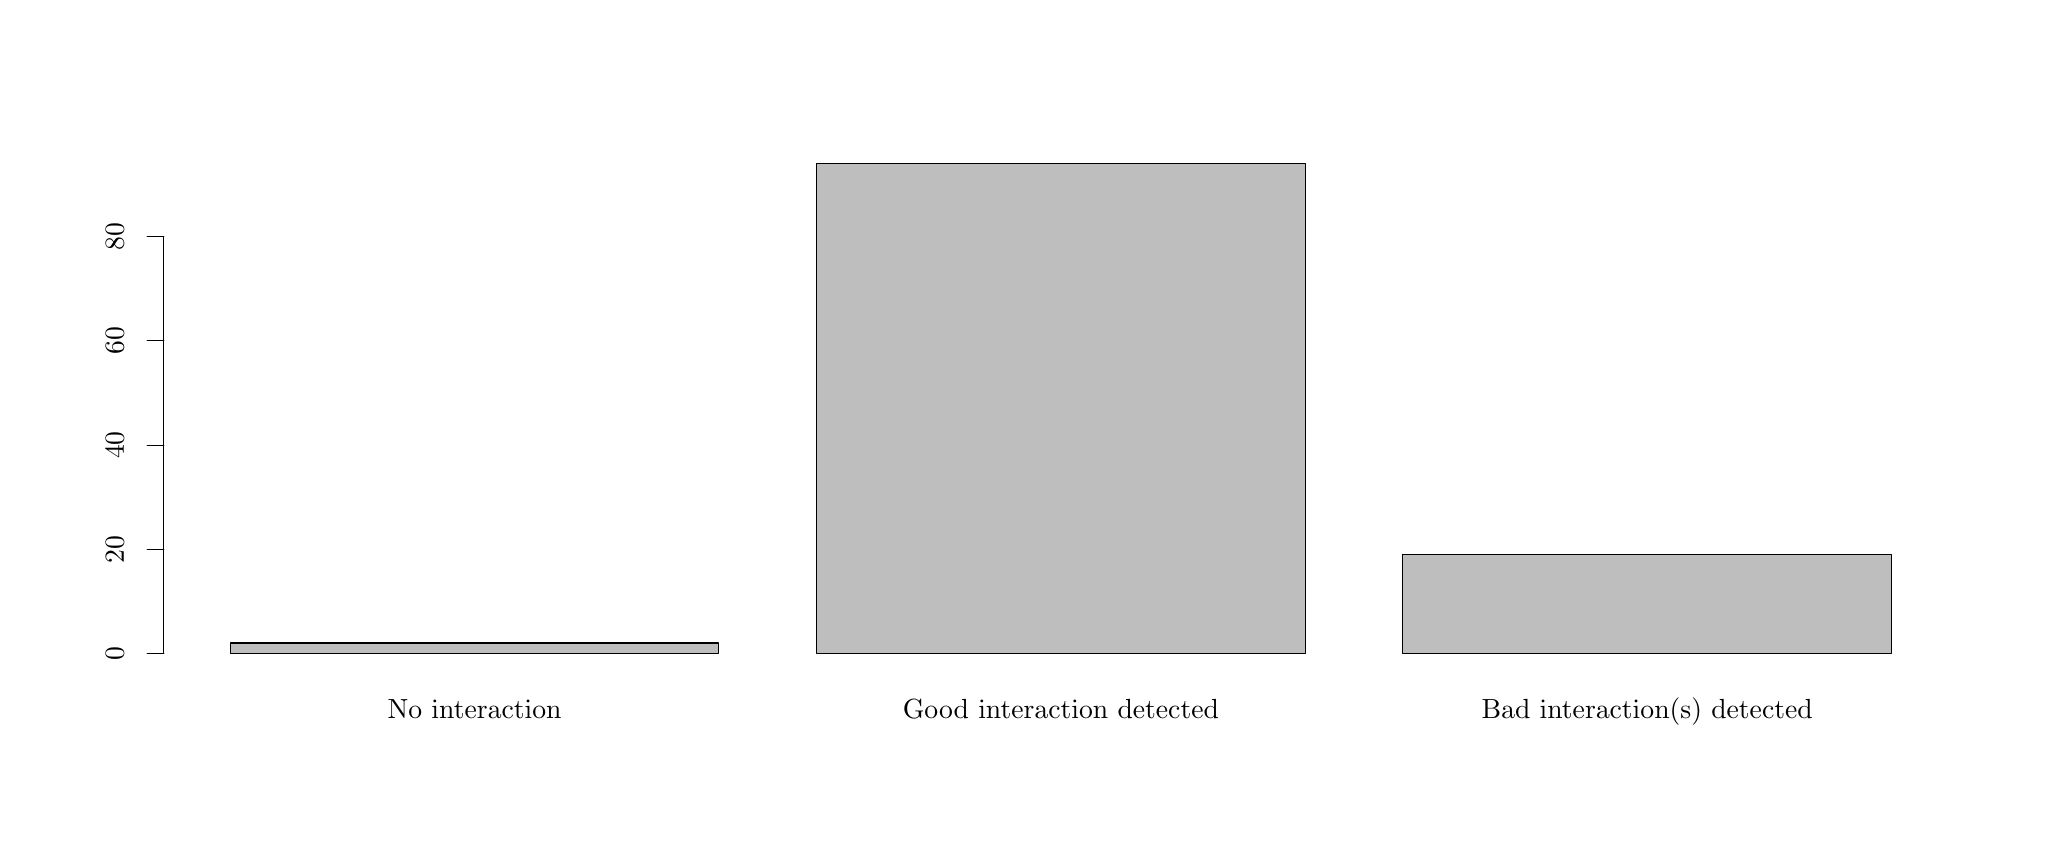
\begin{tikzpicture}[x=1pt,y=1pt]
\definecolor{fillColor}{RGB}{255,255,255}
\path[use as bounding box,fill=fillColor,fill opacity=0.00] (0,0) rectangle (722.70,289.08);
\begin{scope}
\path[clip] (  0.00,  0.00) rectangle (722.70,289.08);
\definecolor{drawColor}{RGB}{0,0,0}
\definecolor{fillColor}{RGB}{190,190,190}

\path[draw=drawColor,line width= 0.4pt,line join=round,line cap=round,fill=fillColor] ( 73.21, 62.97) rectangle (249.76, 66.73);

\path[draw=drawColor,line width= 0.4pt,line join=round,line cap=round,fill=fillColor] (285.07, 62.97) rectangle (461.63,239.88);

\path[draw=drawColor,line width= 0.4pt,line join=round,line cap=round,fill=fillColor] (496.94, 62.97) rectangle (673.49, 98.73);
\end{scope}
\begin{scope}
\path[clip] (  0.00,  0.00) rectangle (722.70,289.08);
\definecolor{drawColor}{RGB}{0,0,0}

\node[text=drawColor,anchor=base,inner sep=0pt, outer sep=0pt, scale=  1.00] at (161.49, 39.60) {No interaction};

\node[text=drawColor,anchor=base,inner sep=0pt, outer sep=0pt, scale=  1.00] at (373.35, 39.60) {Good interaction detected};

\node[text=drawColor,anchor=base,inner sep=0pt, outer sep=0pt, scale=  1.00] at (585.21, 39.60) {Bad interaction(s) detected};

\path[draw=drawColor,line width= 0.4pt,line join=round,line cap=round] ( 49.20, 62.97) -- ( 49.20,213.53);

\path[draw=drawColor,line width= 0.4pt,line join=round,line cap=round] ( 49.20, 62.97) -- ( 43.20, 62.97);

\path[draw=drawColor,line width= 0.4pt,line join=round,line cap=round] ( 49.20,100.61) -- ( 43.20,100.61);

\path[draw=drawColor,line width= 0.4pt,line join=round,line cap=round] ( 49.20,138.25) -- ( 43.20,138.25);

\path[draw=drawColor,line width= 0.4pt,line join=round,line cap=round] ( 49.20,175.89) -- ( 43.20,175.89);

\path[draw=drawColor,line width= 0.4pt,line join=round,line cap=round] ( 49.20,213.53) -- ( 43.20,213.53);

\node[text=drawColor,rotate= 90.00,anchor=base,inner sep=0pt, outer sep=0pt, scale=  1.00] at ( 34.80, 62.97) {0};

\node[text=drawColor,rotate= 90.00,anchor=base,inner sep=0pt, outer sep=0pt, scale=  1.00] at ( 34.80,100.61) {20};

\node[text=drawColor,rotate= 90.00,anchor=base,inner sep=0pt, outer sep=0pt, scale=  1.00] at ( 34.80,138.25) {40};

\node[text=drawColor,rotate= 90.00,anchor=base,inner sep=0pt, outer sep=0pt, scale=  1.00] at ( 34.80,175.89) {60};

\node[text=drawColor,rotate= 90.00,anchor=base,inner sep=0pt, outer sep=0pt, scale=  1.00] at ( 34.80,213.53) {80};
\end{scope}
\end{tikzpicture}

}
\caption{\label{fig:simulated_interaction}Distribution of the kind of interactions chosen by \textit{glmdisc} on 100 simulations.}
\end{figure}




\begin{figure}
\centering
\begin{tikzpicture}
\tikzset{vertex/.style = {shape=circle,draw,minimum size=1.5em}}
\tikzset{edge/.style = {->,> = latex'}}
% vertices
\node[vertex] (x1) at  (0,1.5) {$\glssymbol{X}^1$};
\node[vertex] (xj) at  (0,0) {$\glssymbol{X}^j$};
\node[vertex] (xd) at  (0,-1.5) {$\glssymbol{X}^{d}$};

\node[vertex] (delta) at  (2.5,3) {$\delta$};

\node[vertex] (q1) at  (2.5,1.5) {$Q^1$};
\node[vertex] (qj) at  (2.5,0) {$Q^j$};
\node[vertex] (qd) at  (2.5,-1.5) {$Q^{d}$};

\node[vertex] (y) at (5,0) {$\glssymbol{Y}$};

%edges
\draw[edge] (x1) to (delta);
\draw[edge] (xj) to (delta);
\draw[edge] (xd) to (delta);

\draw[edge] (delta) to (y);

\draw[edge] (x1) to (q1);
\draw[edge] (xj) to (qj);
\draw[edge] (xd) to (qd);
\draw[edge] (q1) to (y);
\draw[edge] (qj) to (y);
\draw[edge] (qd) to (y);

\draw[dashed] (x1) to (xj);
\draw[dashed] (xj) to (xd);

\draw[dashed] (q1) to (qj);
\draw[dashed] (qj) to (qd);
\end{tikzpicture}
\caption{\label{fig:dep}Dépendance entre $\glssymbol{X}^j$,$\E^j$ et $\glssymbol{Y}$} 
\end{figure}




\subsection{Benchmark of \textit{glmdisc} against other approaches} \label{sec:exp}

\subsection{Simulated data from a misspecifed model}

\subsection{Real data from Crédit Agricole Consumer Finance}

\section{Conclusion} \label{sec:ccl}

The essentially industrial problem of introducing pairwise interactions in a supervised multivariate classification setting was formalized and a new approach, relying on a Metropolis-Hastings algorithm has been proposed. This algorithm relies on the use of logistic regression, although other predictive models can be plugged in place of $p_{\glssymbol{bth}}$. (insister là-dessus car toutes les autres approches existantes supposent des modèles)

The true underlying motivation was to perform intetraction screening while quantizing data using the approach developed in the preceding Chapter: \textit{glmdisc}.
The experiments showed that, as was sensed empirically by statisticians in the field of \textit{Credit Scoring}, interactions between quantized features can indeed provide better models than without interactions, or standard logistic regression. This novel approach allows practitioners to have a fully automized and statistically well-grounded tool that achieves better performance than both \textit{ad hoc} industrial practices and academic discretization heuristics at the price of decent computing time but much less of the practitioner's valuable time.

The code used for numerical experiments is available as packages, see Appendix~\ref{app2}.














\printbibliography[heading=subbibliography, title=References of Chapter 4]
